%\textsl{}%!TEX TS-options = --shell-escape
%!TEX TS-program = pdflatex
\documentclass[%
   10pt,              % Schriftgroesse
   nenglish,           % wird an andere Pakete weitergereicht
   a4paper,           % Seitengroesse
   DIV11,             % Textbereichsgroesse (siehe Koma Skript Dokumentation !)
]{scrartcl}%     Klassen: scrartcl, scrreprt, scrbook, article
% -------------------------------------------------------------------------

\usepackage[utf8]{inputenc} % Font Encoding, benoetigt fuer Umlaute
\usepackage[english]{babel}   % \textsl{}Spracheinstellung

\usepackage[T1]{fontenc} % T1 Schrift Encoding
\usepackage{textcomp}    % Zusatzliche Symbole (Text Companion font extension)
\usepackage{lmodern,dsfont}     % Latin Modern Schrift
\usepackage{dsfont}
\usepackage{color}
%\usepackage{wasysym}
\usepackage{ulem}
\usepackage{graphicx}
\usepackage{grffile} %allows to use pngs
%\usepackage{epstopdf} % allows to use eps
\usepackage{eurosym}
%\usepackage{txfonts}
\usepackage{stmaryrd}
\usepackage{amsfonts}
\usepackage{amsmath}
\usepackage{mathtools}
\usepackage{hyperref}
\usepackage{tikz}
\usepackage{multirow}
\usepackage{listings}
\usepackage{etextools}
\usepackage{ifthen}
\usepackage{cite}
%\usepackage{TikZ} %phylogenetischer Baum
%\usetikzlibrary{calc, shapes, backgrounds} %für die Phylogenetische bäume
%\usetikzlibrary{automata,arrows}
\usepackage{subfigure} 


% Definition des Headers
\usepackage{geometry}
\geometry{a4paper, top=3cm, left=3cm, right=3cm, bottom=3cm, headsep=0mm, footskip=0mm}
\renewcommand{\baselinestretch}{1.3}\normalsize

\def\header#1#2#3#4#5#6#7{\pagestyle{empty}
\noindent
\begin{minipage}[t]{0.6\textwidth}
\begin{flushleft}
\textbf{#4}\\% Fach
#6\\% Semester
Tutor: #2  % Tutor 
\end{flushleft}
\end{minipage}
\begin{minipage}[t]{0.4\textwidth}
\begin{flushright}
\points{#7}% Punktetabelle
\vspace*{0.2cm}
#5%  Names
\end{flushright}
\end{minipage}

\begin{center}
{\Large\textbf{ Assignment #1}} % Blatt

{(Handed in #3)} % Abgabedatum
\end{center}
}

\newenvironment{vartab}[1]
{
    \begin{tabular}{ |c@{} *{#1}{c|} } %\hline
}{
    \end{tabular}
}

\newcommand{\myformat}[1]{& #1}

\newcommand{\entry}[1]{
  \edef\result{\csvloop[\myformat]{#1}}
  \result \\ \hline
}

\newcommand{\numbers}[1]{
  \newcounter{ctra}
\setcounter{ctra}{1}
\whiledo {\value{ctra} < #1}%
{%
  \myformat{\thectra}
  \stepcounter{ctra}%
}
\myformat{\thectra}
}
\newcommand{\emptyLine}[1]{
  \newcounter{ctra1}
\setcounter{ctra}{1}
\whiledo {\value{ctra1} < #1}%
{%
  \myformat{\hspace*{0.5cm}}
  \stepcounter{ctra1}%
}
}

\newcommand{\points}[1]{
\newcounter{colmns}
\setcounter{colmns}{#1}
\stepcounter{colmns}
  \begin{vartab}{\thecolmns}
    \numbers{#1} & $\sum$ (6)\\\hline   %add here Complete number of points ---------------------------
    \emptyLine{\thecolmns}\\
  \end{vartab}
}


\begin{document}
%\header{Blatt}{Tutor}{Abgabedatum}{Vorlesung}{Bearbeiter}{Semester}{Anzahl Aufgaben}
\header{7}{Alexander Seitz}{30. November 2015}{Bioinformatics I}{\\Jonas Ditz \\\& Benjamin Schroeder}{WS 15/16}{2}

\section*{Practical Assignment - \textsl{Planted Motif Problem Generator}}
A executable .jar-File of the written program for this task is attached to the our hand-in. The .jar can be executed via a commandline with the command "java -jar SeqGen.jar". The help for usage can be called with the option "-h", "-help", "--help" or "-?". Generally we tried to be as user-friendly as possible, via using options as input markers and generating detailed and clear error messages, if a input is invalid or missing. General needed input values are the options "-k <int>" ammount of sequences in the final set, "-n <int>" the sequence length, "-d <int>" the amount of deviation positions and "-l <int>" the length of the motif  or "-M <String>" a motif itself. If "-l <int>" is entered, a random motif is generated. With "-M <String>" the String is used as motif and "-l" is of course not needed, and vice versa. The "-o <String>" option is optional and stand for the output name. If no option is added the test run is started with the default values from the assignment sheet.\\
 The motifs are generated with d deviation positions, which are not independent from each other. So if d is 2, there are two variable positions in the motif. These can not fall onto the same position. But each position can deviate as one of all four basic nucleotides, so also as the one which was already contained.\\
 Another feature of our program is, that it also generates sequences with based on an amino acid alphabet. Switching to the amino acids the option "-E p" is needed. For the basicDNA bases no option is needed, although there is the "-E n" option. Also a matter of user-friendliness is the fact of never overwriting the output, but instead counting up an number. This causes the comfort of never overwriting accidently a file.

\section*{Practical Assignment - \textsl{MEME and Gibbs sampler}}

\subsection*{Method}
We used two different software solution of Motif finder to perform a Motif search on our test sets. 
The first tool was MEME-suite \cite{meme} a set of Motif-based sequence analysis tools. For this task 
we used the online implementation of MEME\footnote{http://meme-suite.org/tools/meme} with the site 
distribution parameter set to ``One occurrence per sequence'' and the number of Motifs set to one. 
On the other hand we used the Gibbs Motif Sampler \cite{gibbs}. All parameters were set to their 
default values except we set the -n flag to use nucleic acid alphabet.

All test sets of sequences used for this task were generated by SeqGen. This is a self-programmed 
Java tool, which uses four parameters to build a set of sequences. A overview of important parameters 
of SeqGen can be found in table \ref{tab:params}. We generated five different test sets (see table 
\ref{tab:sets}), which we used for comparison of MEME and Gibbs sampler.

\begin{table}[ht]
 \centering
 \caption{Parameters of SeqGen}
 \begin{tabular}{|l|l|}
  \hline
  Parameter & Description \\
  \hline
  k & number of sequences \\
  n & length of each sequence \\
  l & length of Motif \\
  d & number of deviating positions \\
  M & specify a Motif (optional) \\
  \hline
 \end{tabular}
 \label{tab:params}
\end{table}

\begin{table}[ht]
 \centering
 \caption{parameter, which was used to generated test sets}
 \begin{tabular}{|c|c|c|c|c|c|}
  \hline
    & k & n & l & d & M \\
  \hline
  test set 1 & 20 & 100 & 10 & 2 & AGTGGAACAG \\
  test set 2 & 15 & 150 & 15 & 3 & CTTTGAGCAAATAAT \\
  test set 3 & 20 & 100 & 5 & 1 & ATATC \\
  test set 4 & 25 & 50 & 5 & 2 & CTGCA \\
  test set 5 & 25 & 100 & 10 & 1 & ACAGGGGTGC \\
  \hline
 \end{tabular}
 \label{tab:sets}
\end{table}

\subsection*{Result}

MEME was able to find a Motif for all of the five test sets (see Figure \ref{fig:memeLogo}). However, 
one can see easily that it overestimated the length for short Motifs. 

\begin{figure}[ht]
 \centering
 \subfigure[test set 1]{
  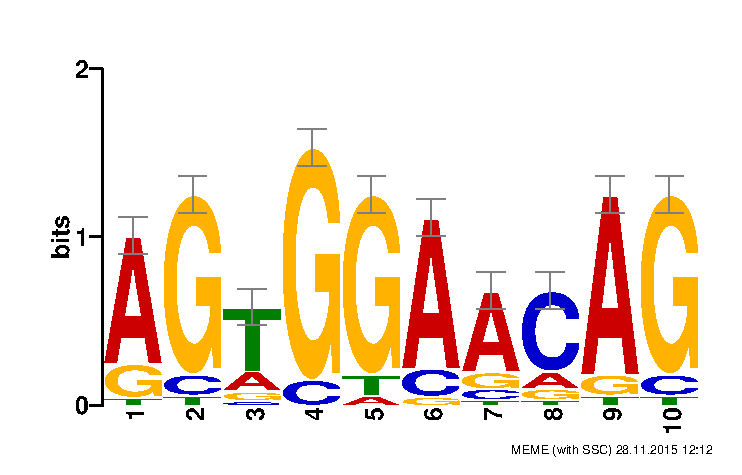
\includegraphics[width=0.45\textwidth]{results_MEME/logo_testSetVorgabe}
 }
 \subfigure[test set 2]{
  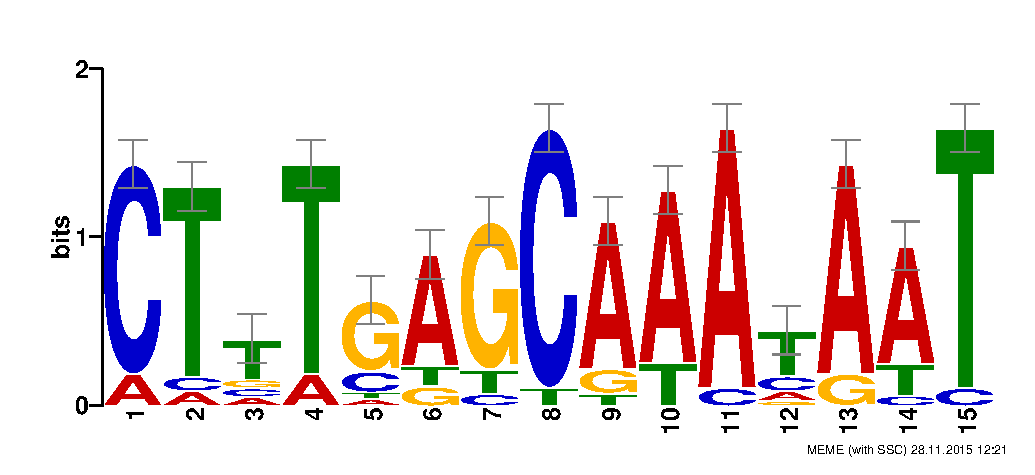
\includegraphics[width=0.45\textwidth]{results_MEME/logo_testSet1}
 }
 \subfigure[test set 3]{
  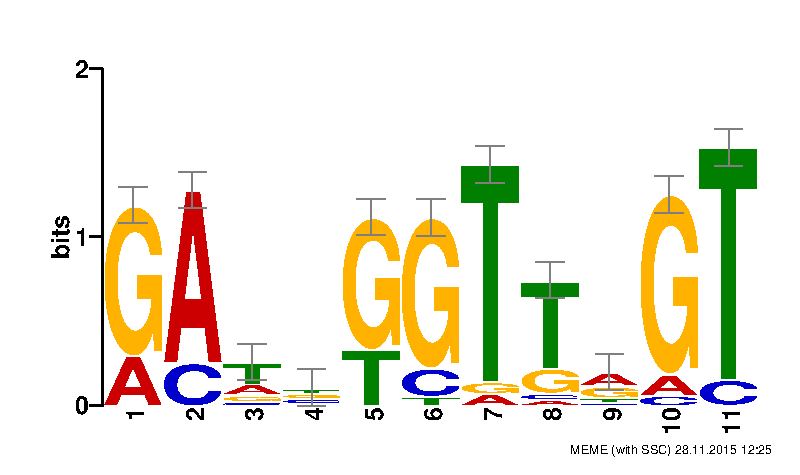
\includegraphics[width=0.45\textwidth]{results_MEME/logo_testSet2}
 }
 \subfigure[test set 4]{
  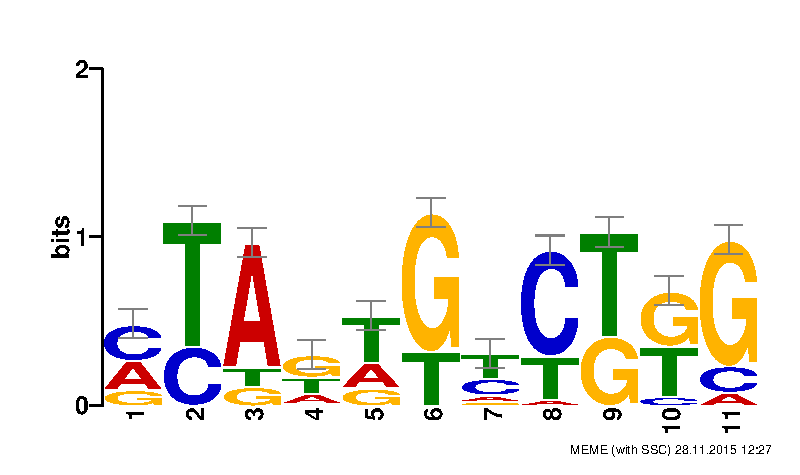
\includegraphics[width=0.45\textwidth]{results_MEME/logo_testSet3}
 }
 \subfigure[test set 5]{
  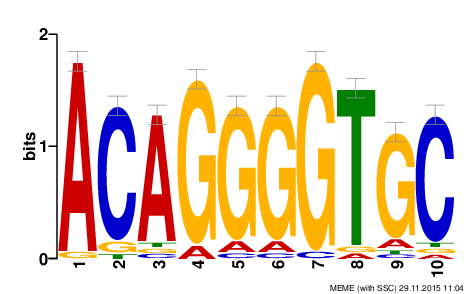
\includegraphics[width=0.45\textwidth]{results_MEME/logo_testSet4}
 }
 \caption{Sequence logo of calculated Motifs by MEME}
 \label{fig:memeLogo}
\end{figure}

Even worst was the result of Gibbs sampler. This program was only able to find the Motif in test set 
two and five. For all of the three other sets, Gibbs sample could not find any Motif in the sequences
(see table \ref{tab:gibbsResult}).

\begin{table}[ht]
 \centering
 \caption{Detected Motifs by Gibbs sampler. The letter N means that Gibbs sampler did not give a suggestion for this position.}
 \begin{tabular}{|l|l|}
  \hline
    & Motif \\
  \hline
  test set 1 & \textit{No Motifs detected} \\
  test set 2 & ANTNTTNGCTNANAG \\
  test set 3 & \textit{No Motifs detected} \\
  test set 4 & \textit{No Motifs detected} \\
  test set 5 & TACAGGGGTNC \\
  \hline
 \end{tabular}
 \label{tab:gibbsResult} 
\end{table}

If we compare the runtime of both programs (see table \ref{tab:runtime}) one can see that MEME is in 
general a little bit faster. But since we used the webservice of MEME and run Gibbs sampler on a local 
machine with a single core CPU and just one Gb of RAM, the comparability of theses runtimes may not 
be given.

\begin{table}
 \centering
 \caption{Runtime of used programs in Seconds}
 \begin{tabular}{|c|c|c|}
  \hline
    & MEME & Gibbs sampler \\
  \hline
  test set 1 & 1.66 & 1.04 \\
  test set 2 & 3.33 & 1.13 \\
  test set 3 & 1.66 & 1.05 \\
  test set 4 & 1.66 & 0.78 \\
  test set 5 & 3.33 & 1.19 \\
  \hline
 \end{tabular}
 \label{tab:runtime}
\end{table}


\subsection*{Discussion}

With the results given above one can see that both, MEME and Gibbs sampler, have a problem with 
Motifs of too small size. Since the Motif finding problem is not statistically solvable for small 
Motifs\cite{bioinf1}, this observation makes sense. Also MEME seems to have a higher sensitivity, 
since it still find a Motif for test set three and four but a wrong one. Obviously for these wrong 
Motifs the position found by MEME were also wrong but for all other Motifs MEME found the exact 
positions. On the other hand Gibbs sampler has a lower sensitivity than MEME and it also did not 
output the positions of the founded Motifs. So it is difficult to proof that Gibbs sampler found 
the right Motifs.

Under the circumstances discussed above and with respect to the much more user-friendly interface of 
MEME-Suite we would recommend to use that website.

\newpage
\bibliography{Assignment7-Ditz_Schroeder-WS15-16.bib}
\bibliographystyle{ieeetr}
 
\end{document}
